%Punchline!

%make plot of delta [C/N] versus R0(1D), color code observed binned points by mass of the star

Given the measured amounts of mixing described in Section \ref{sec:obs} and the reduced density ratios $r$ computed for stars of various masses and metallicities described in Section \ref{sec:mesa_results}, it is now possible to compare the observed %\sout{amounts of} 
extra mixing to the predictions of various thermohaline models from Section \ref{sec:formalism} and assess whether the observed mixing is at least qualitatively consistent with \textbf{any such theoretical prescription.}
%that which would be driven by the thermohaline instability.
%
We show in Figure \ref{Fig:punchline} the corrected changes in [C/N] compared to the inferred reduced density ratios, in an orientation analogous to the theoretical predictions shown in Figure \ref{fig:parameterization_compare}. We note that the observed trends are not strongly sensitive to the assumed mixing model, {as we find that mixing decreases with increasing reduced density ratio} no matter which parameterization is chosen. 


Interestingly, the data show both similarities and differences compared to the theoretical prescriptions, shown again in Figure \ref{Fig:compare} for comparison. The observed mixing is strongly correlated with the fluid parameters as predicted, even for stars with different masses and metallicities but similar reduced density ratios. %\textbf{This is} consistent with theoretical predictions under the simplifying assumption that the mixing efficiency and magnetic field are not varying strongly with mass or metallicity. 
We note a decrease in the amount of mixing as the density ratio increases, which is %\textbf{once again}
consistent with standard prescriptions of \textbf{thermohaline} mixing but inconsistent with the prescription informed by 3D magnetohydrodynamic %\sout{models} \sout{\textbf{formulations}}\red
simulations that include strong magnetic fields. We also note that the range of reduced density ratios probed by the observational data we have available here is much smaller than the range of density ratios simulated by and studied within the theoretical 3D fluid dynamics community \red{AF add citation}. As such, we must be cognizant of the limitations of our data coverage; for instance, the observations do not probe the high-$r$ regimes where magnetic fields are most important. %\sout{suggesting that focusing simulations on the relevant range might be beneficial.} %, assuming the density ratios inferred in this paper are assumed correctly.   

%observations do not probe high values of the reduced density ratios where magnetic fields may be important

%note that the scatter is also important here- if the mixing actually depends on B field, and that depends randomly on the star (or on the stellar M/Z combo on average), then stars of the same R0 should have a range of mixi-ness. If R0 is the only parameter that matters, then mixing should strongly correlate with R0 with only minimal/ observational measurement scatter. 

%FIGURE solar---------------------------------------------------
\begin{figure*}[!tb]
\begin{center}
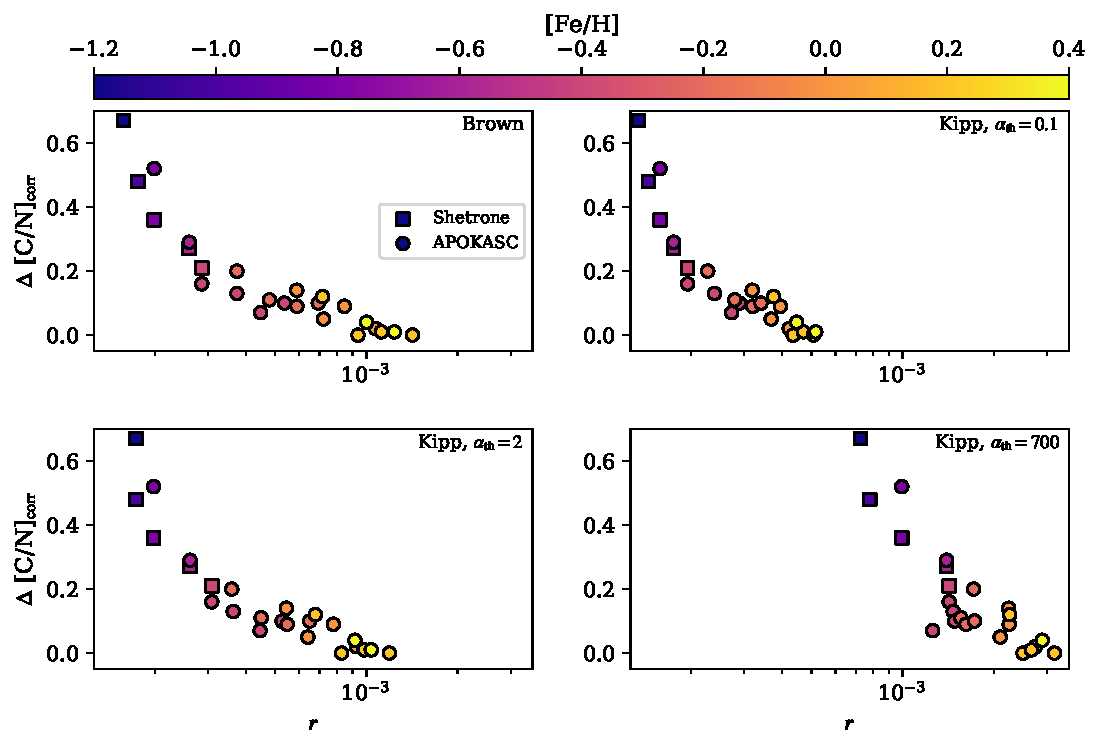
\includegraphics[width=\textwidth]{mixing_vs_r.pdf}%[width=9cm, clip=true, trim=1in 1in 1in 1in]{./Figs/omgcomp.eps}
\caption{Corrected measurements of the change in [C/N] near the red giant branch bump, compared to the reduced density ratio inferred from one-dimensional models using various thermohaline mixing prescriptions (Brown, Kippenhahn $\alpha_{\rm th}=0.1$, Kippenhahn $\alpha_{\rm th}=0.2$,Kippenhahn $\alpha_{\rm th}=0.700$), color coded by the metallicity bin of each data point. In general, there is a clear correlation between these parameters, suggesting that the observed mixing is related to the unstable mean molecular weight gradient. Mixing and the reduced density ratio $r$ are inversely correlated, which is consistent with hydrodynamic thermohaline prescriptions. \sout{More mixing is observed when the fluid is more \textbf{unstable to the thermohaline instability [can this be said a different way?]}; this is consistent with standard theories of thermohaline mixing.} We note that the observations do not probe high values of the reduced density ratios, which is where magnetic fields are most important. \red{EA Add delta cn$_cor$}
\label{Fig:punchline}
}
\end{center}
\end{figure*}

\begin{figure*}[!tb]
\begin{center}
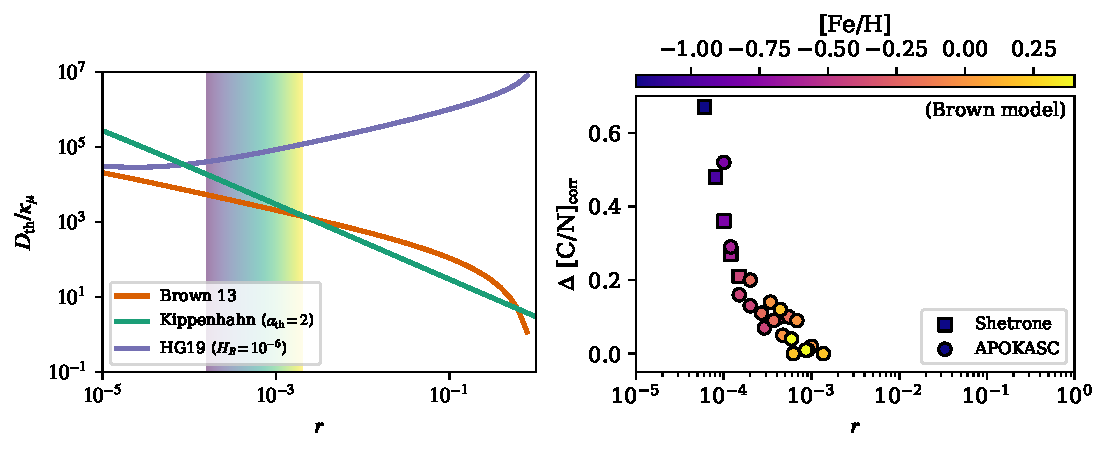
\includegraphics[width=\textwidth]{punchline.pdf}
\caption{\textbf{Left:} A reproduction of Figure \ref{fig:parameterization_compare} showing the predicted rate of mixing versus the reduced density ratio in various prescriptions of thermohaline mixing, including hydrodynamic (orange, green) and magnetohydrodynamic (purple) models. \textbf{Right:} The observed extra mixing near the red giant branch bump as a function of the reduced density ratio inferred from one dimensional stellar evolution models. While the conversion from the change in a mixing diagnostic to the fluid mixing rate is not trivial, and therefore we do not attempt it here, we note that the observed mixing amounts are strongly negatively correlated with $r$, with stars probing on average a relatively narrow range of the regime formally unstable to thermohaline mixing. }
\label{Fig:compare}
\end{center}
\end{figure*}


